\section*{Introduction}

A distributed system is made highly available when individual servers are
allowed to operate independently without coordination that may be prone to
failure or high latency.
The independent nature of the server's behavior means that it can immediately
respond to client requests, but that it does so from a limited, local
perspective which may be inconsistent with another server's response.
If individual servers in a system were allowed to remain wholly independent,
individual requests from clients to different servers would create a lack of
order or predictability, a gradual decline into inconsistency, e.g. the
system would experience \textit{entropy}.
To combat the effect of entropy while still remaining highly available,
servers engage in \textit{anti-entropy sessions}~\cite{terry_session_1994} at
a routine interval, a process that occurs in the background of client
requests.

Anti-entropy sessions synchronize the state between servers ensuring that,
at least briefly, the local state is consistent with a portion of the global
state of the system.
If all servers engage in anti-entropy sessions, the system is able to make
some reasonable guarantees about the timeliness of responses; the most famous
of which is that in the absence of requests the system will become
consistent, eventually.
More specifically, inconsistencies in the form of stale reads can be bound by
likelihoods that are informed by the latency of anti-entropy sessions and the
size of the system~\cite{bailis_quantifying_2014}.
Said another way, overall consistency is improved in an eventually consistent
system by decreasing the likelihood of a stale read, which is tuned by
improving the \textit{visibility latency} of a write, the speed at which a
write is propagated to a significant portion of servers.
This idea has led many system designers to decide that ``eventual consistency
is consistent enough''~\cite{bermbach_eventual_2011,wada2011data}
particularly in a data center context where visibility latency is far below
the rate of client requests, leading to practically strong consistency.

More recently there have been two important changes in

\section*{System Description}

A basic sketch of an eventually consistent system is as follows:

\section*{Bandit Approaches}

\section*{Experiments}

\begin{figure*}[t]
    \centering
    \minipage{0.5\textwidth}
      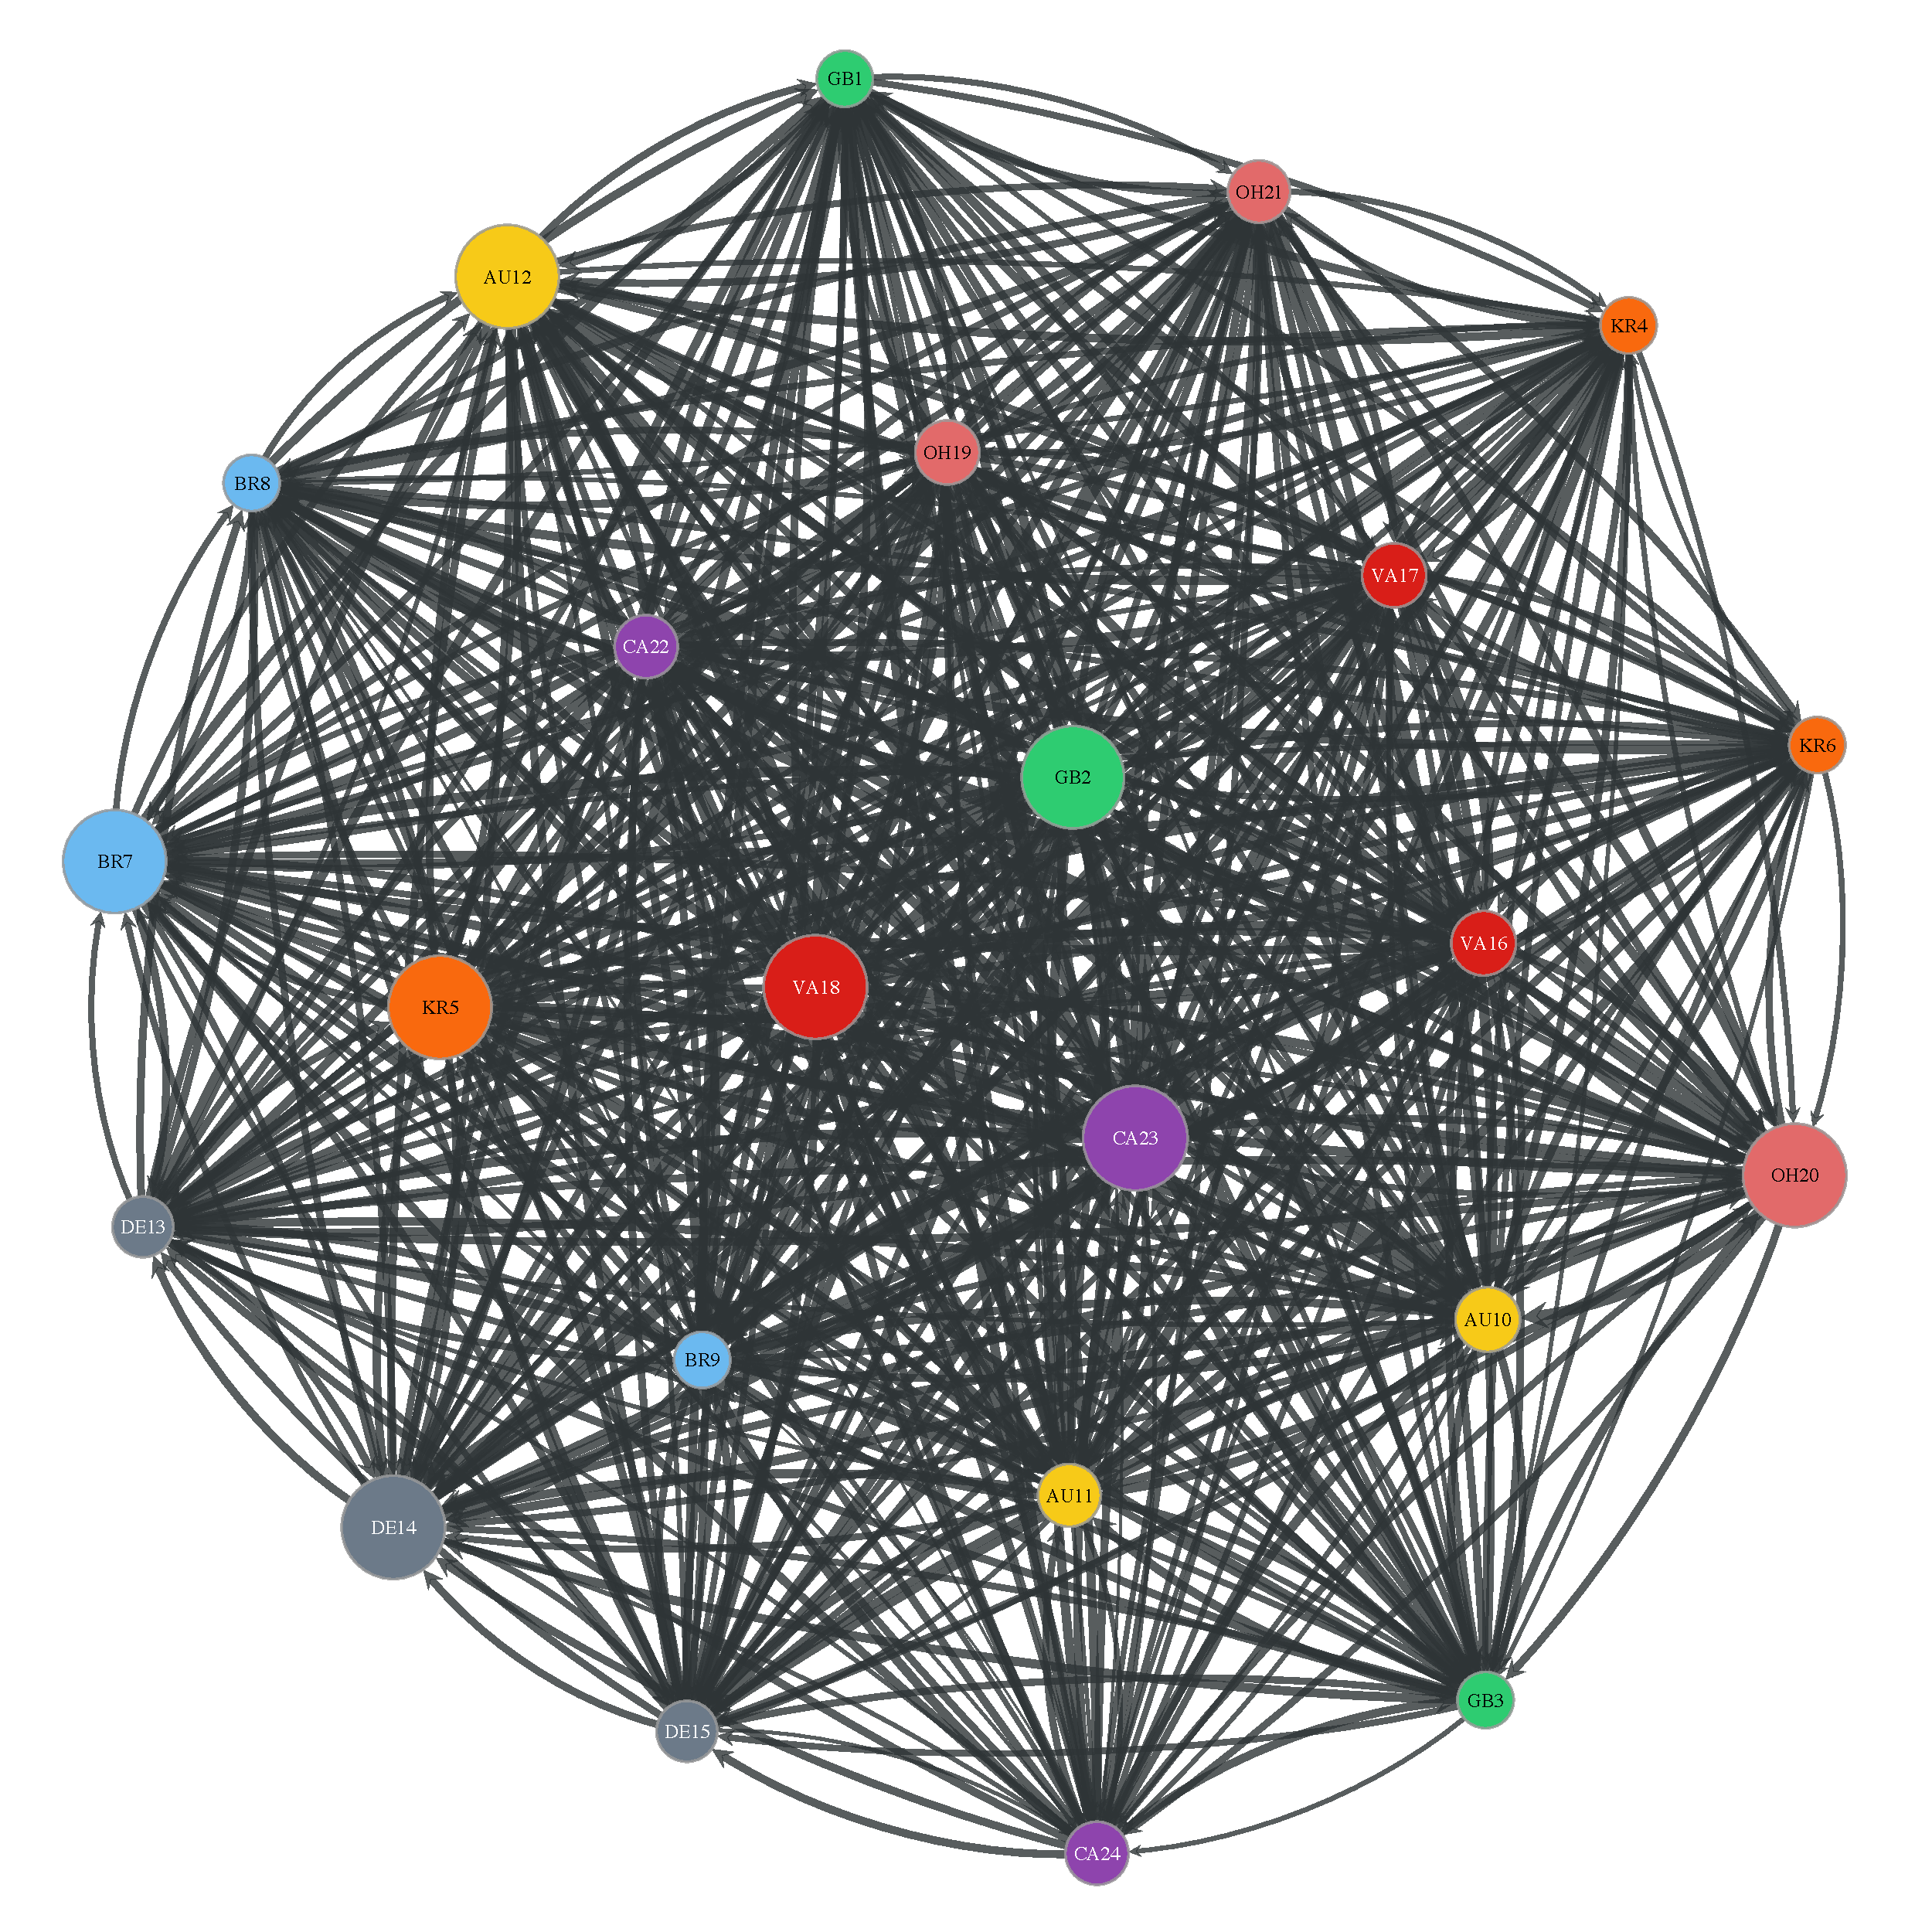
\includegraphics[width=\linewidth]{figures/b-uniform-selection-e1}
      \caption{Uniform Selection}\label{fig:uniform_selection}
    \endminipage\hfill
    \minipage{0.5\textwidth}%
      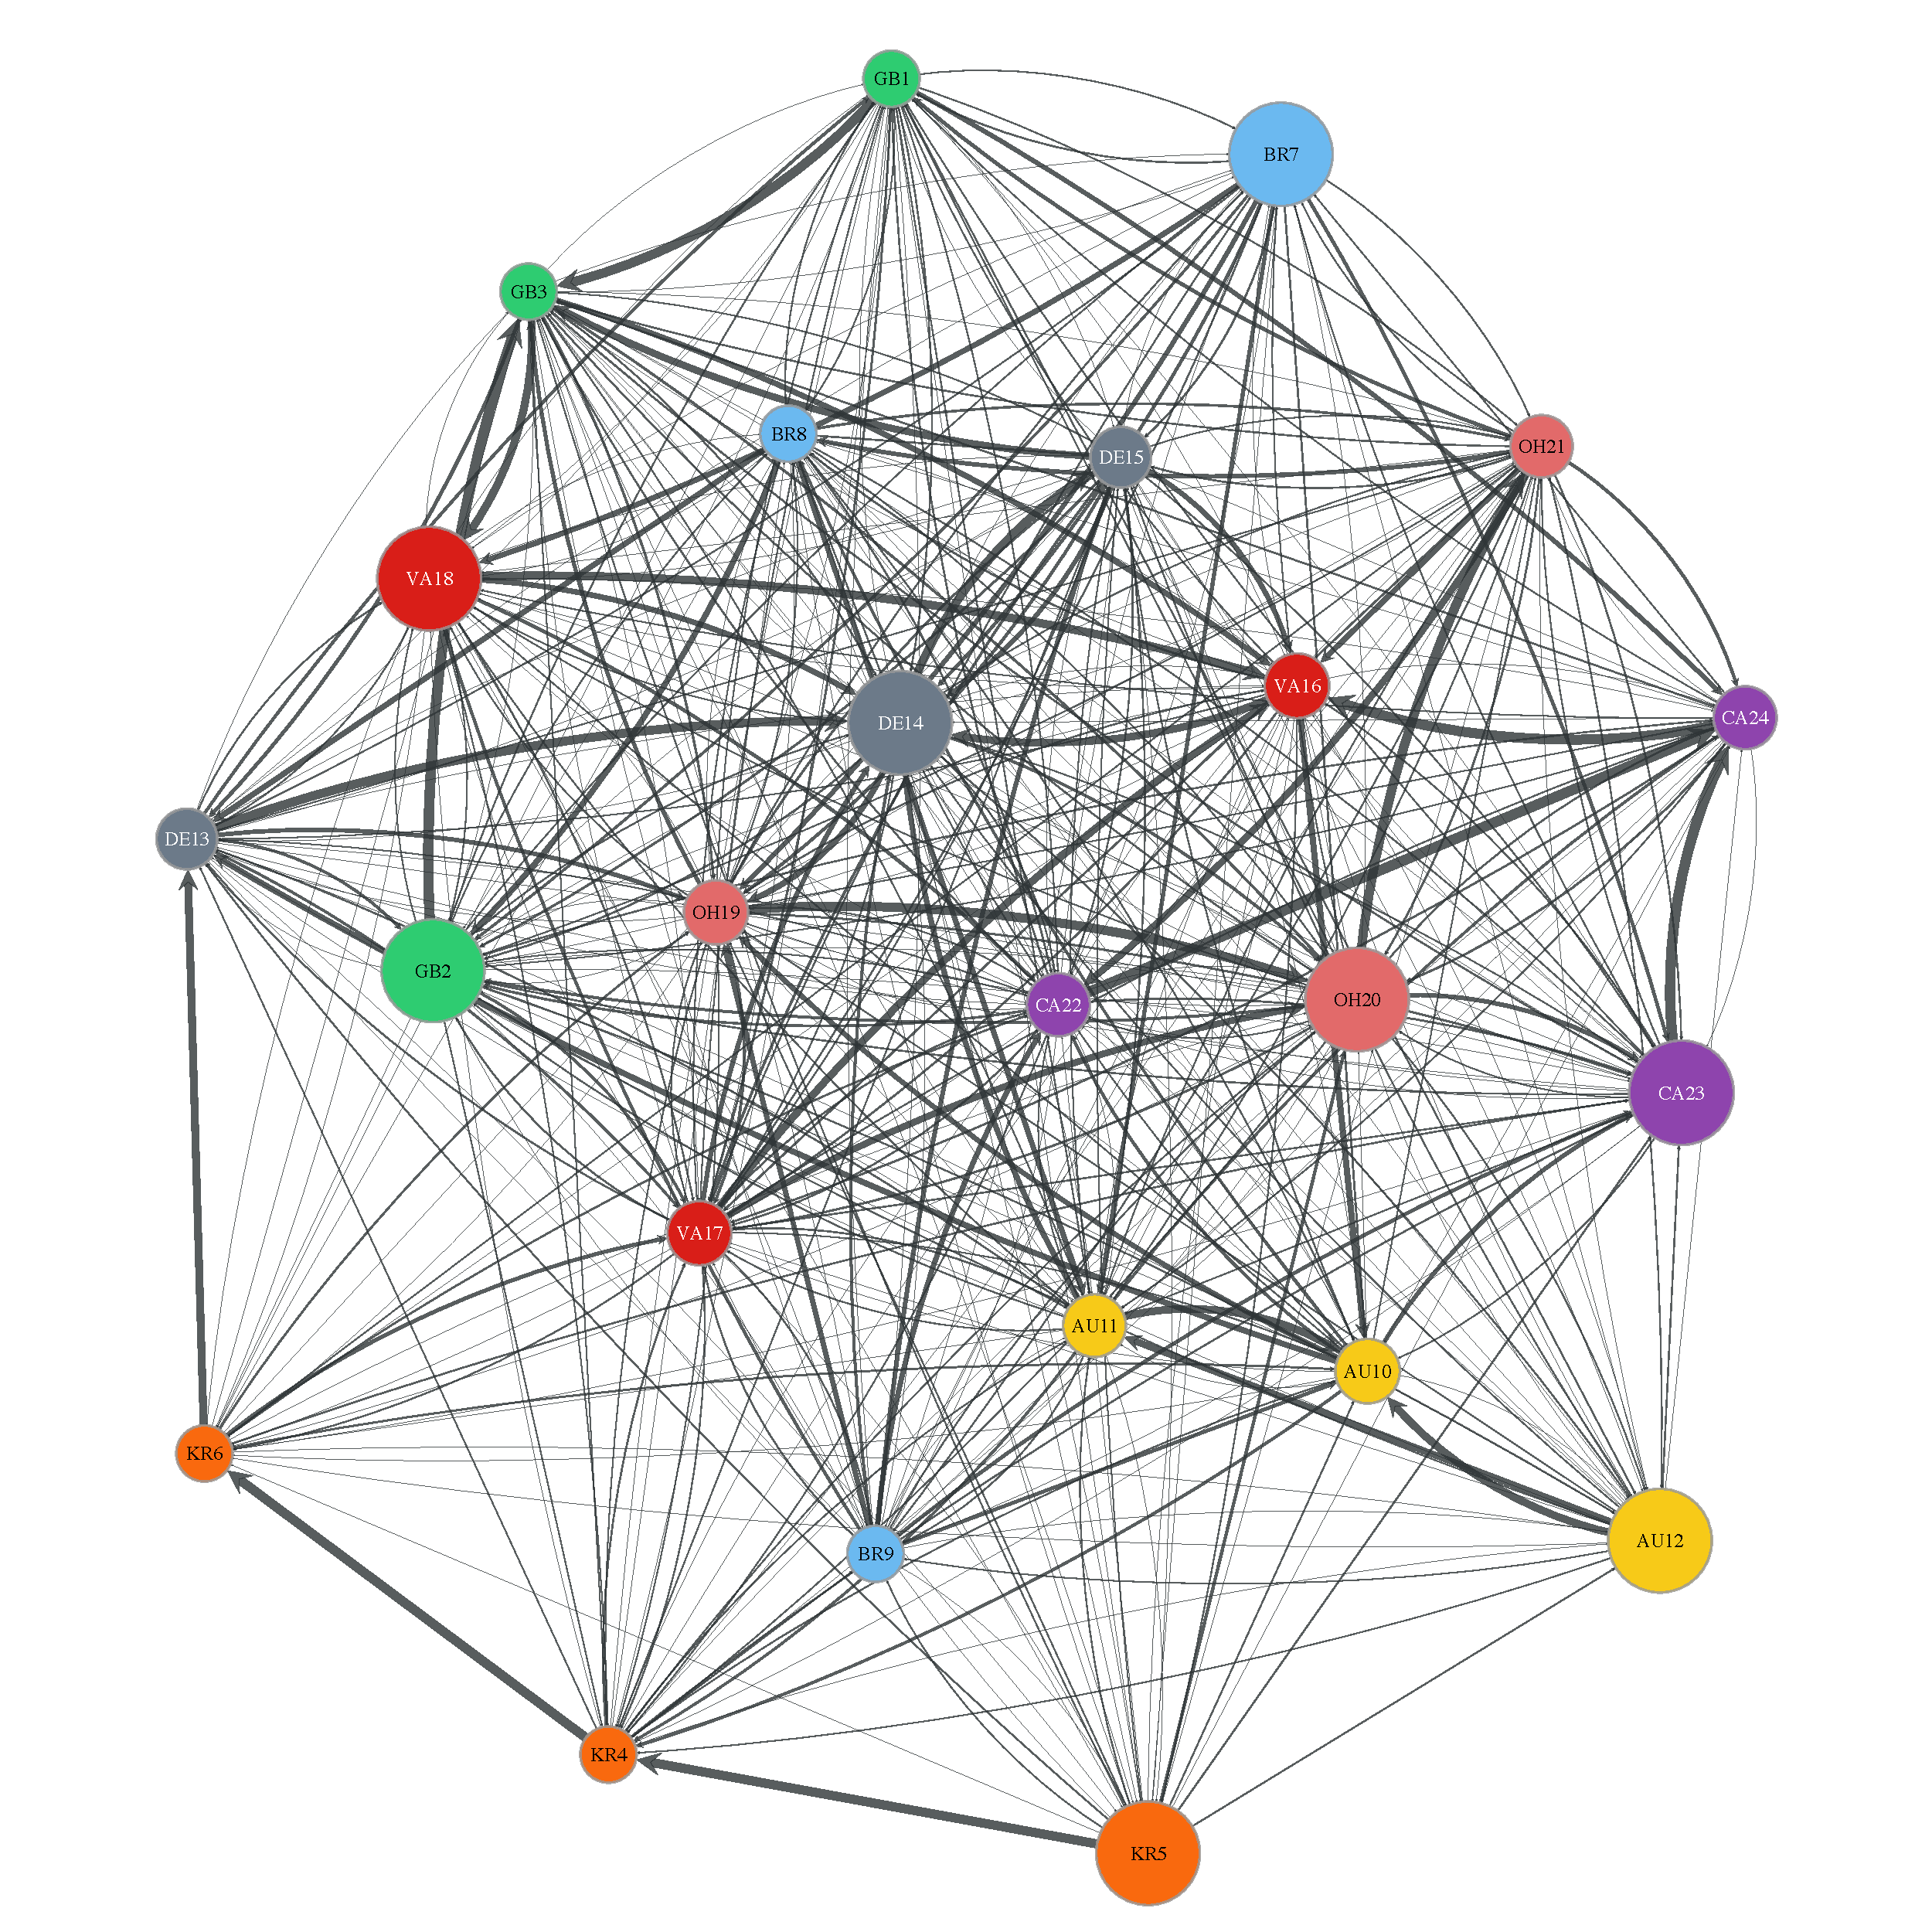
\includegraphics[width=\linewidth]{figures/b-epsilon-greedy-0-1-e2}
      \caption{Epsilon Greedy $\epsilon=0.1$}\label{fig:epsilon_greedy_e1}
    \endminipage
\end{figure*}

\begin{figure*}[t]
    \centering
    \minipage{0.5\textwidth}%
      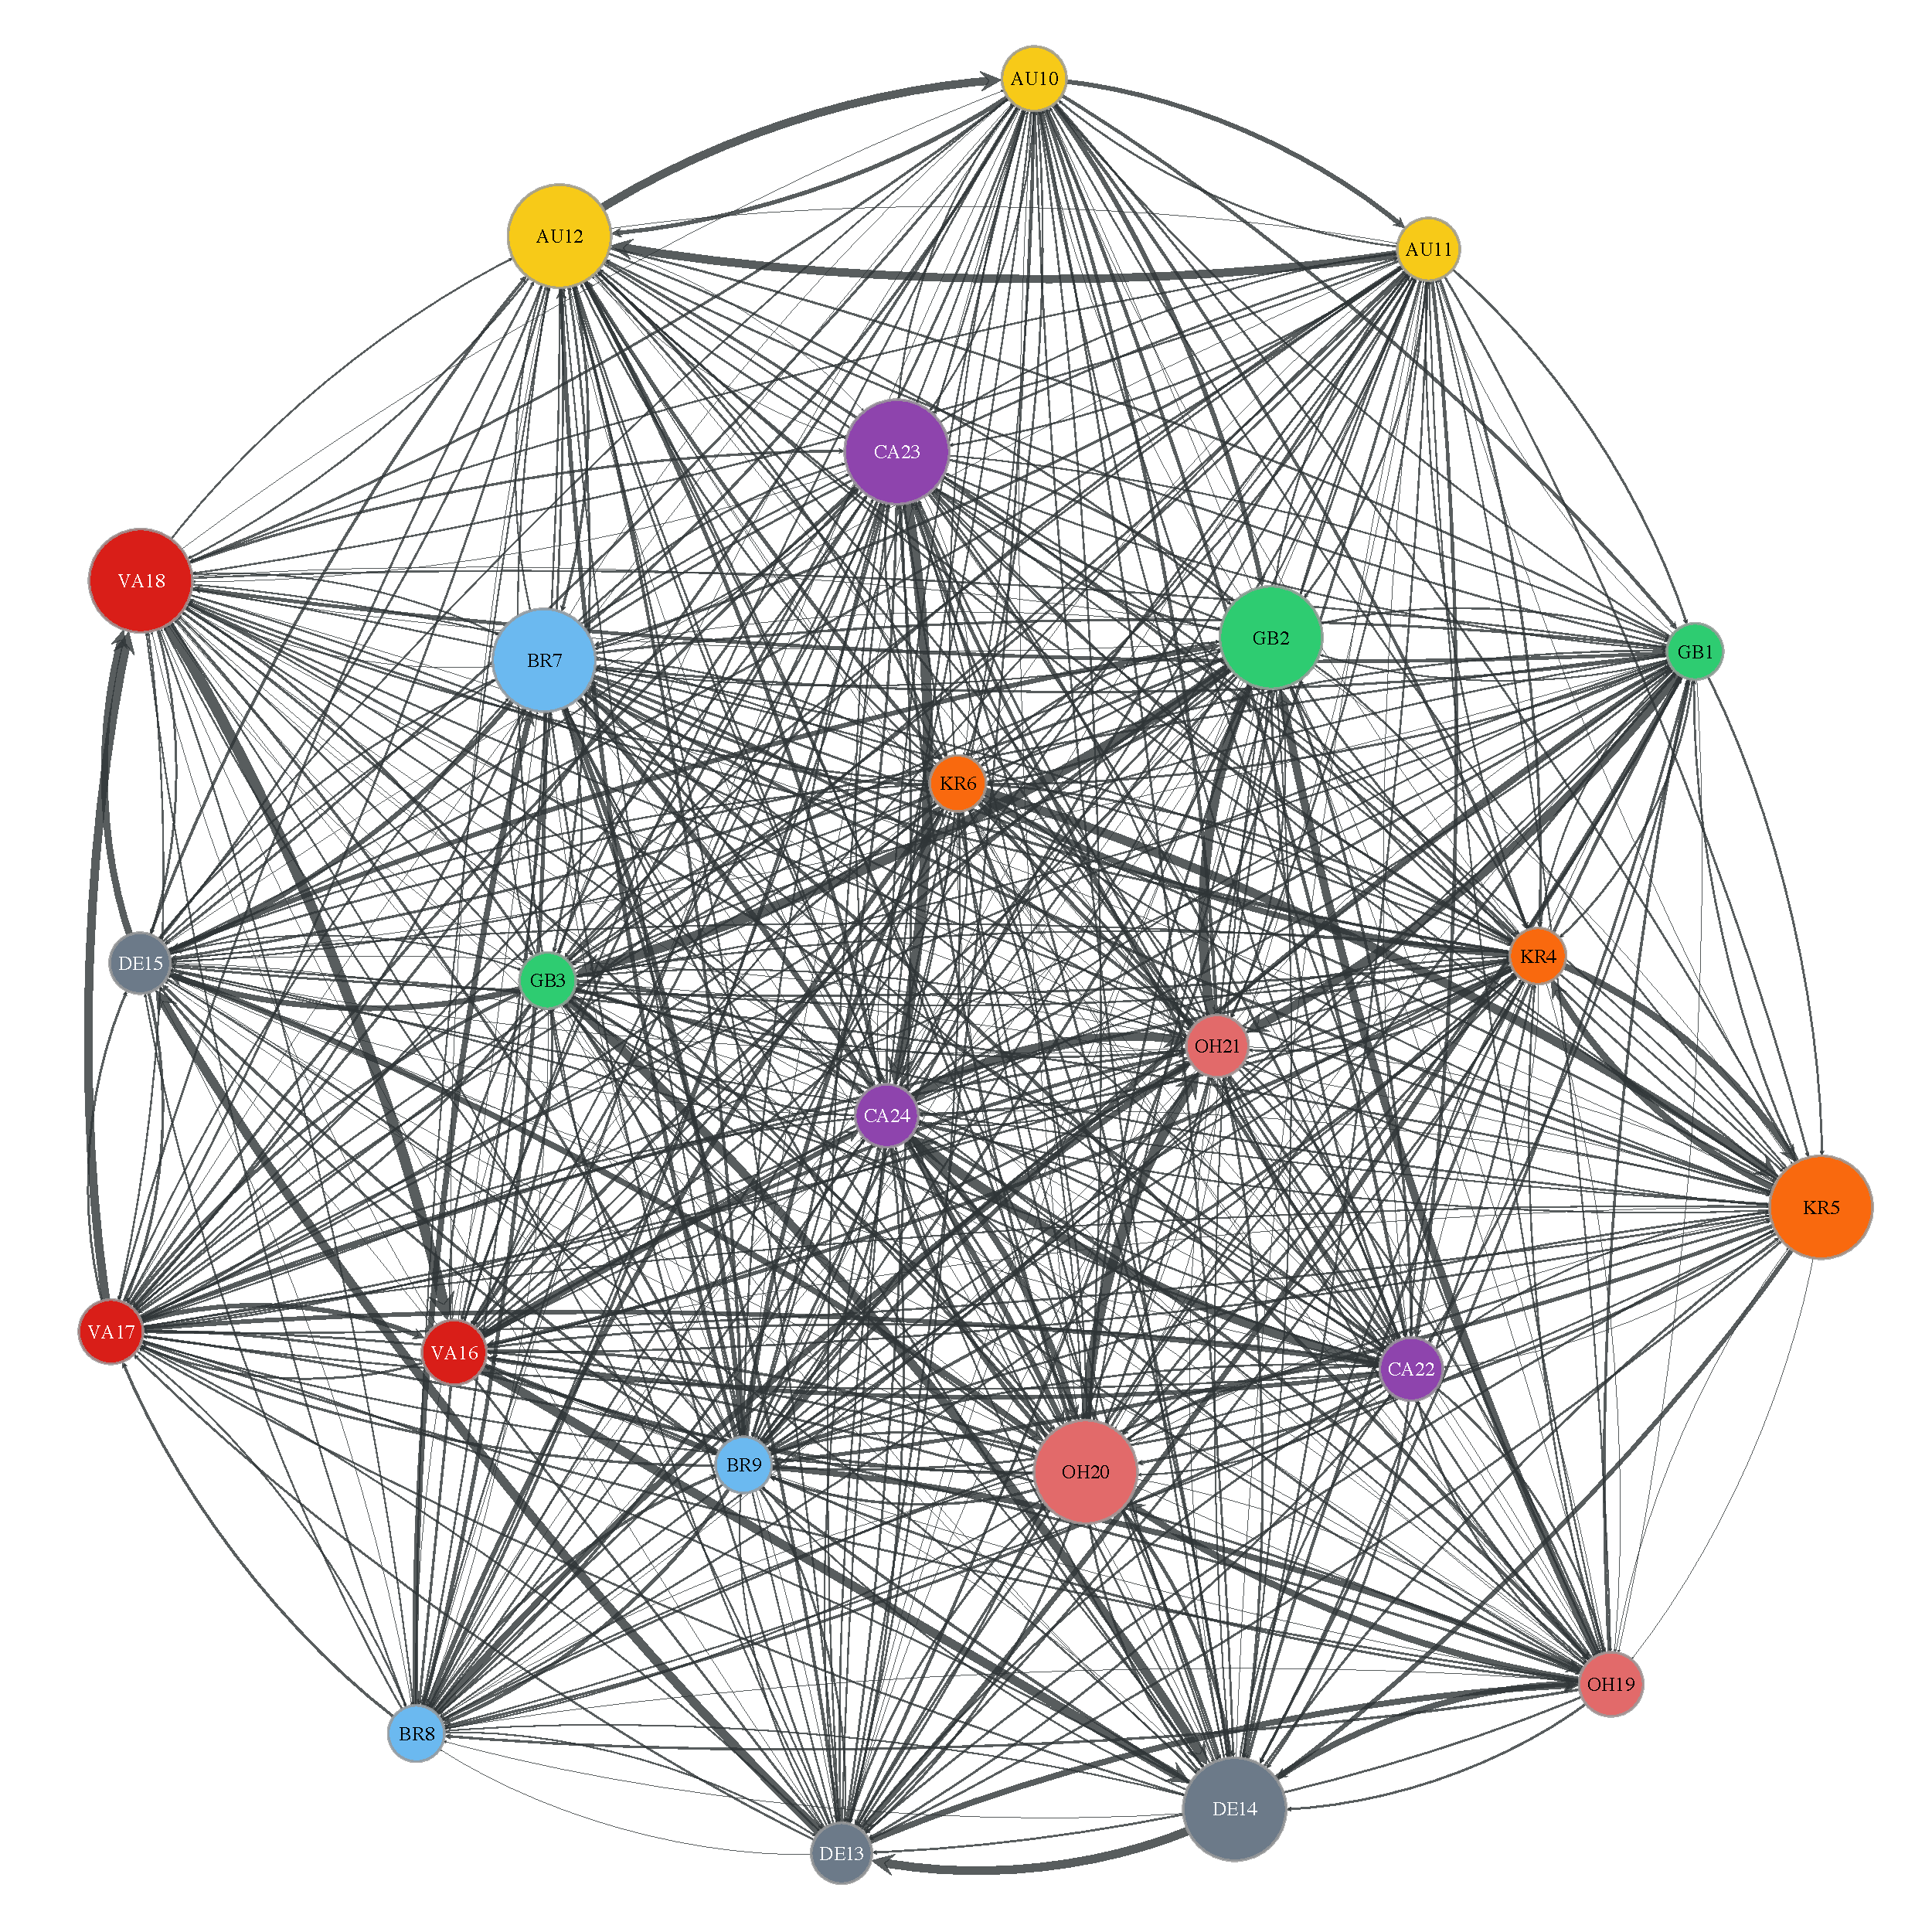
\includegraphics[width=\linewidth]{figures/b-epsilon-greedy-0-2-e3}
      \caption{Epsilon Greedy $\epsilon=0.2$}\label{fig:epsilon_greedy_e2}
  \endminipage\hfill
  \minipage{0.5\textwidth}%
    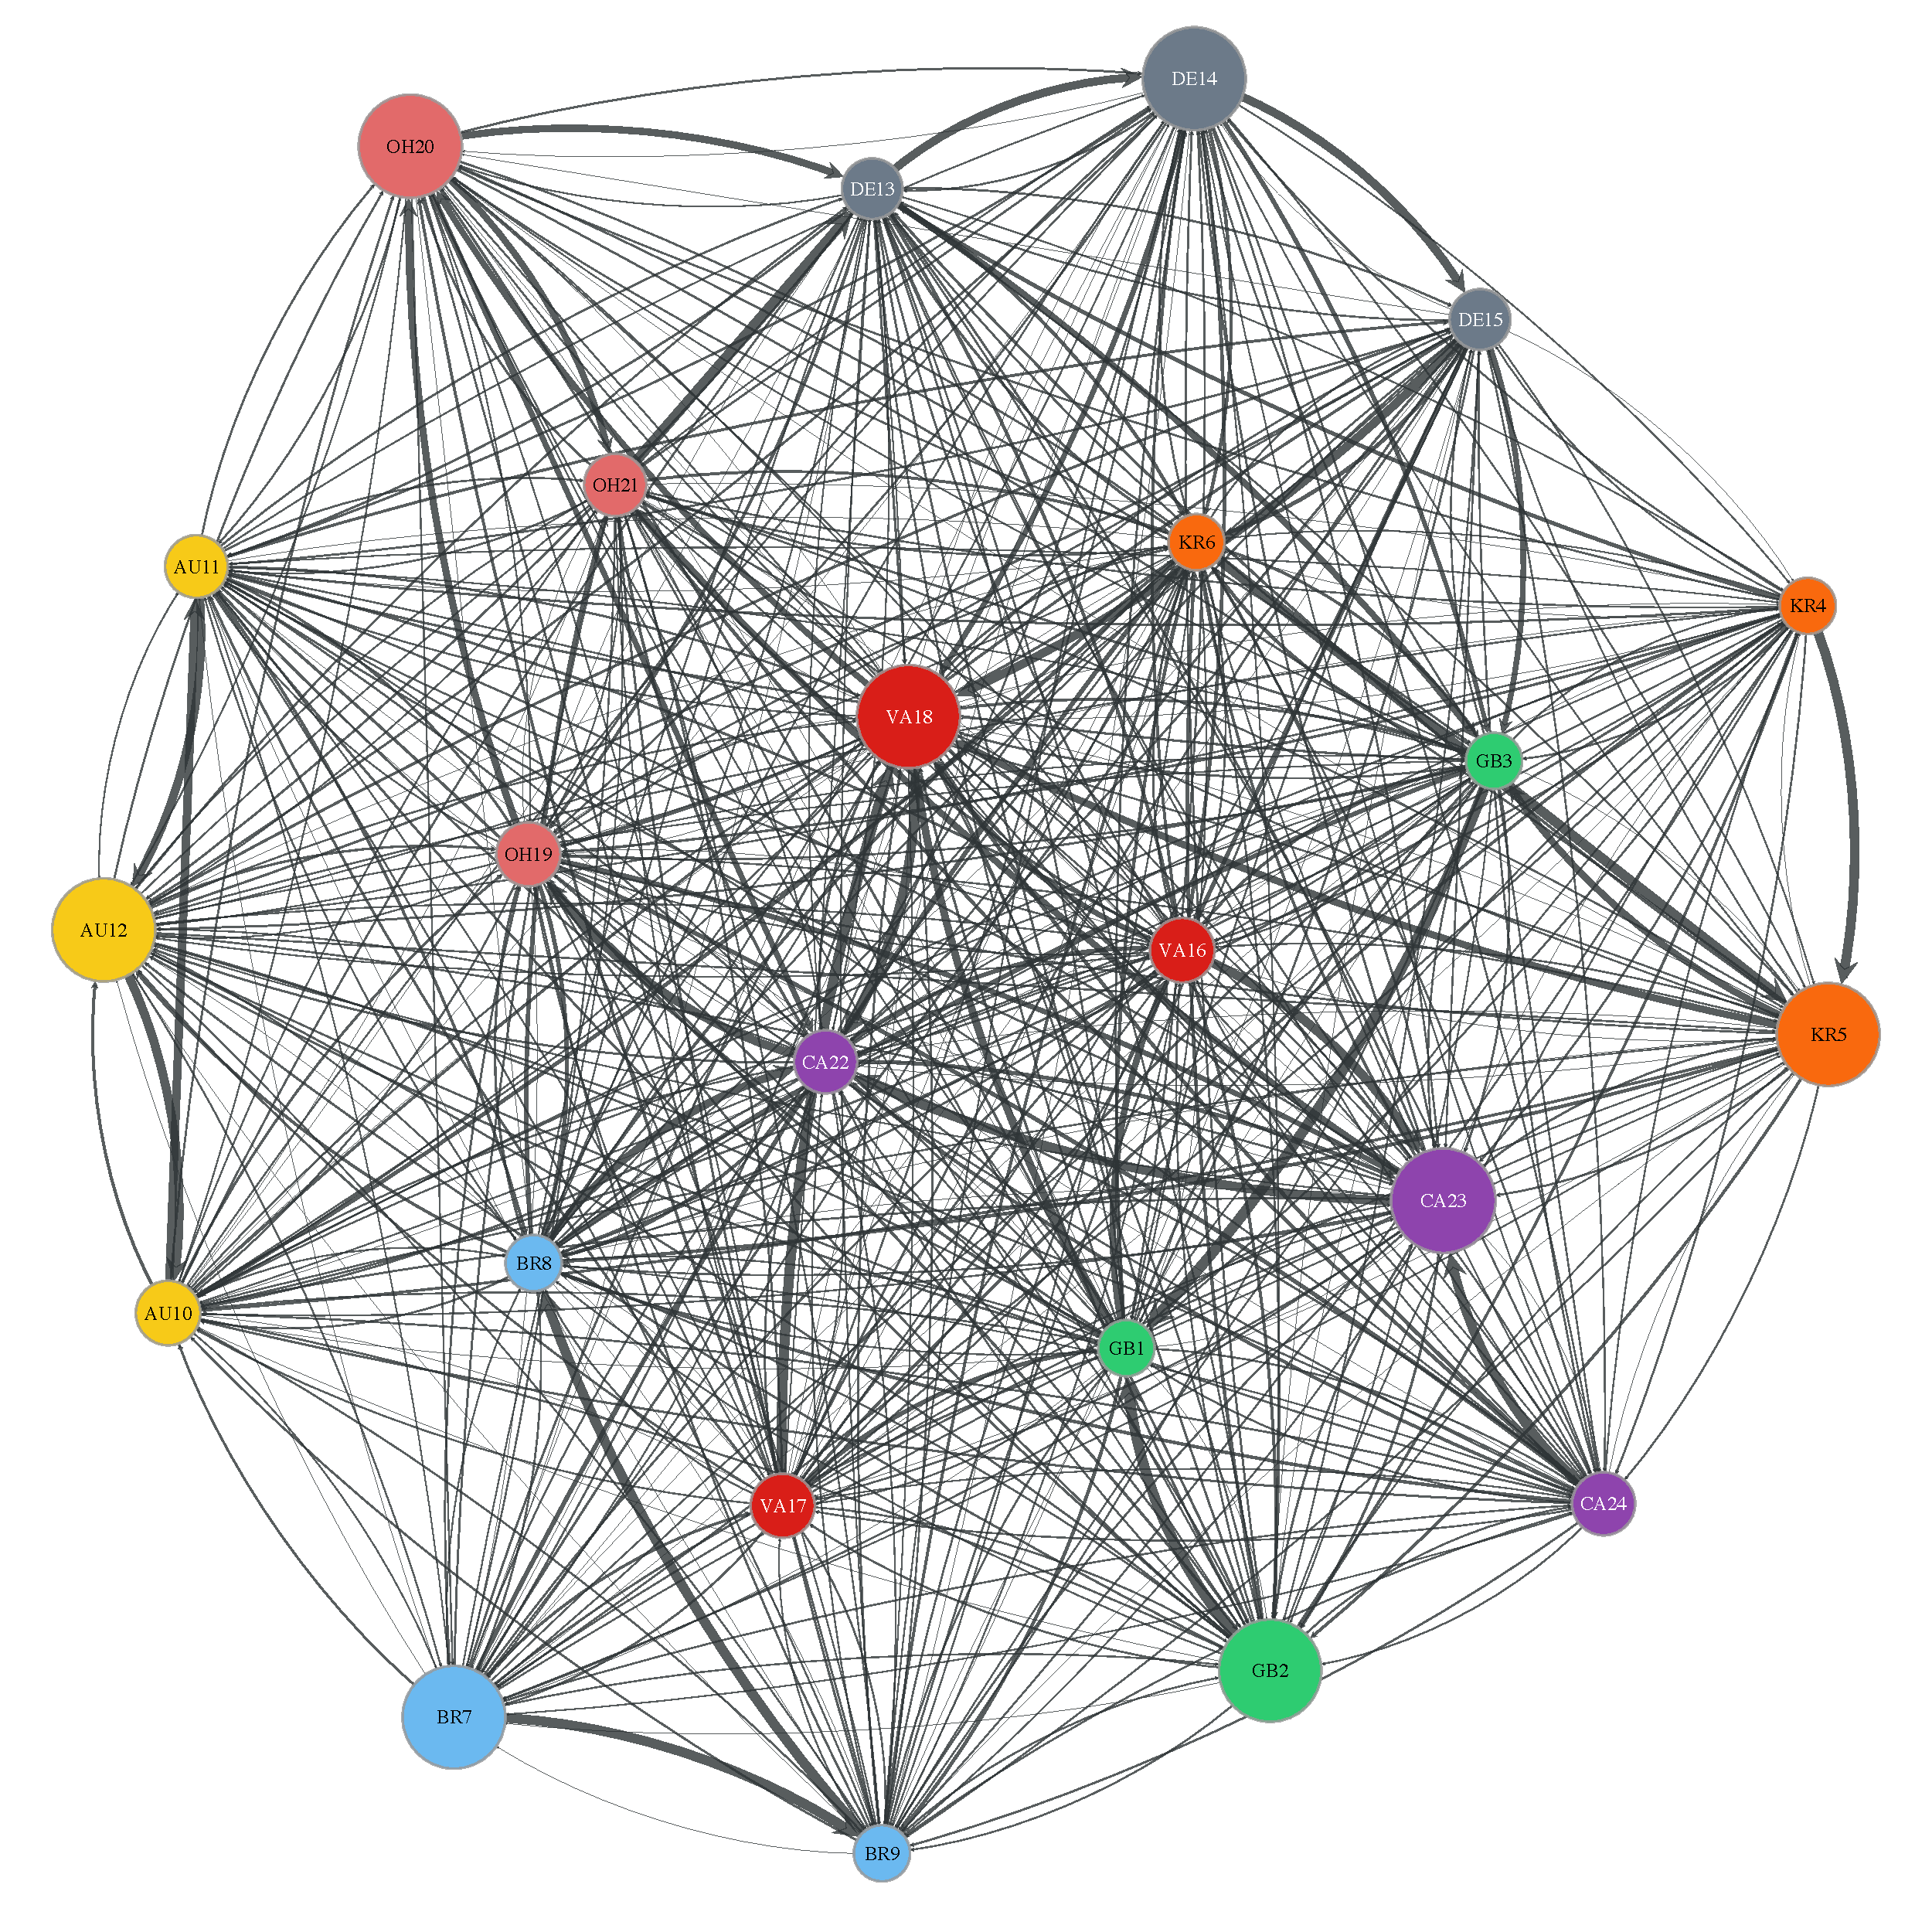
\includegraphics[width=\linewidth]{figures/b-annealing-epsilon-greedy-e5}
    \caption{Annealing Epsilon}\label{fig:annealing_epsilon}
  \endminipage
\end{figure*}


\section*{Discussion}

\section*{Conclusion}

% \begin{acks}
% The authors would like to thank the servers for working so hard.
% \end{acks}
